% !TeX encoding = UTF-8
\chapter{Task 3: Data Pre-processing}\label{chap:task3_preprocessing}

The task asks us to analyze the labels, handle infinite and NaN values, scale the features with min-max scaling and select the 20 best features with \texttt{SelectKBest}. We implemented this in Python 3.12 with pandas and scikit-learn~\cite{pedregosa2011sklearn} (module \texttt{data.py}, \texttt{features.py} and the script \texttt{task3\_preprocess.py}). The steps are, in this order:

\begin{enumerate}\setlength\itemsep{0pt}
	\item \textbf{Load and analyze labels.} 65 of the 79 column names carry stray leading spaces and are stripped. The en dash in the attack labels was stored as an invalid byte and decodes as U+FFFD (``\texttt{Web Attack \char"FFFD{} XSS}''). We read the file as UTF-8 with replacement, map that character to ``-'' and collapse whitespace. Every label is validated against the four expected classes.
	\item \textbf{Drop the duplicate column.} \texttt{Fwd Header Length} appears twice in the header, a known artifact of the CICFlowMeter export. We drop the second copy.
	\item \textbf{Infinity and NaN.} We replace $\pm\infty$ by NaN and \emph{drop} the affected rows. Only 135 rows (0.08\,\%) are affected, all of them BENIGN, so dropping loses no attack information and introduces no artificial values. The infinite values occur only in \texttt{Flow Bytes/s} and \texttt{Flow Packets/s}: CICFlowMeter divides by the flow duration, which is 0 for single-packet flows.
	\item \textbf{Duplicate rows.} We remove exact duplicates before splitting. Otherwise identical rows land in both train and test sets and inflate the test scores.
	\item \textbf{Constant columns.} They carry no information and trigger warnings in \texttt{SelectKBest}.
	\item \textbf{Identical columns.} Columns equal to an earlier one (tolerance $10^{-6}$) are removed, so that the 20 selected features are distinct. The tolerance is needed for one pair, \texttt{Bwd Packet Length Mean} and \texttt{Avg Bwd Segment Size}: they are the same quantity but differ in 2 rows by $10^{-6}$ because of CSV rounding.
	\item \textbf{Train/test split.} A stratified 70/30 split on the four-class label with \texttt{random\_state=42}, done \emph{before} anything is fitted. Both targets, binary (BENIGN vs.\ ATTACK) and multiclass, use the same split.
	\item \textbf{Min-max scaling.} \texttt{MinMaxScaler(clip=True)} maps each feature to $[0,1]$. It is fitted on the training set only, so no test statistics leak into training, and \texttt{clip=True} keeps unseen values, such as live traffic later, inside $[0,1]$.
	\item \textbf{Feature selection.} \texttt{SelectKBest(chi2, k=20)} on the scaled training set, once per target. We scale first because $\chi^2$ requires non-negative input, and the raw data contains negative values: \texttt{Init\_Win\_bytes\_*} is $-1$ when no window was observed, and a few durations are negative.
\end{enumerate}

The column-level steps 5 and 6 use feature values only, never labels, so they leak no label information. Listing~\ref{lst:clean} shows the core of steps 2--6 in the code.

% U+FFFD in line 40 of data.py would otherwise leak into the first listing line (listings/LuaTeX quirk)
{\catcode"FFFD=9 \lstinputlisting[style=py,float=htbp,linerange={117-119,121-121,132-136,139-143,146-150,153-157},caption={Core cleaning steps of \texttt{clean()} in \texttt{src/lab2ids/data.py} (steps 2--6; logging calls omitted)},label={lst:clean}]{../src/lab2ids/data.py}}

\section{Results}\label{sec:t3-results}

Table~\ref{tab:t3cleaning} lists the cleaning steps with their effect, and Table~\ref{tab:t3removed} the removed columns. The 14 of the 6,066 duplicate rows of the raw file that contain infinite or NaN values were already removed in step 3, which leaves 6,052 for step 4. The six bulk-transfer features are always 0 in this CICFlowMeter version. Notably, \texttt{Fwd PSH Flags} is identical to \texttt{SYN Flag Count}, although these are different TCP flags. This points to a feature-extraction problem in the CICFlowMeter version used for CIC-IDS2017, in line with the literature~\cite{engelen2021troubleshooting}.

\begin{table}[ht]
	\centering\small
	% AUTO-GENERATED by scripts/make_report_tables.py from outputs/task3/cleaning_report.json -- do not edit
\begin{tabularx}{\linewidth}{rlrrX}
\toprule
\# & Step & Rows & Cols & Detail \\
\midrule
1 & Drop duplicate header column & 170\,366$\to$170\,366 & 79$\to$78 & $-$1 column (\texttt{Fwd Header Length.1}) \\
2 & Replace $\pm\infty$ by NaN & 170\,366$\to$170\,366 & 78$\to$78 & inf: \texttt{Flow Bytes/s} 115, \texttt{Flow Packets/s} 135; NaN: \texttt{Flow Bytes/s} 20 \\
3 & Drop NaN rows & 170\,366$\to$170\,231 & 78$\to$78 & $-$135 rows (all BENIGN) \\
4 & Drop duplicate rows & 170\,231$\to$164\,179 & 78$\to$78 & $-$6\,052 rows (6\,015 BENIGN, 37 Brute Force) \\
5 & Drop constant columns & 164\,179$\to$164\,179 & 78$\to$68 & $-$10 columns \\
6 & Drop identical columns & 164\,179$\to$164\,179 & 68$\to$61 & $-$7 columns \\
\midrule
 & \textbf{Result} & \textbf{164\,179} &  & \textbf{164\,179 rows $\times$ 60 features} \\
\bottomrule
\end{tabularx}

	\caption{Cleaning steps. The column counts include the \texttt{Label} column, so the 61 remaining columns are 60 features plus \texttt{Label}. Loading and label fixing happen before step 1.}
	\label{tab:t3cleaning}
\end{table}

\begin{figure}[ht]
	\centering
	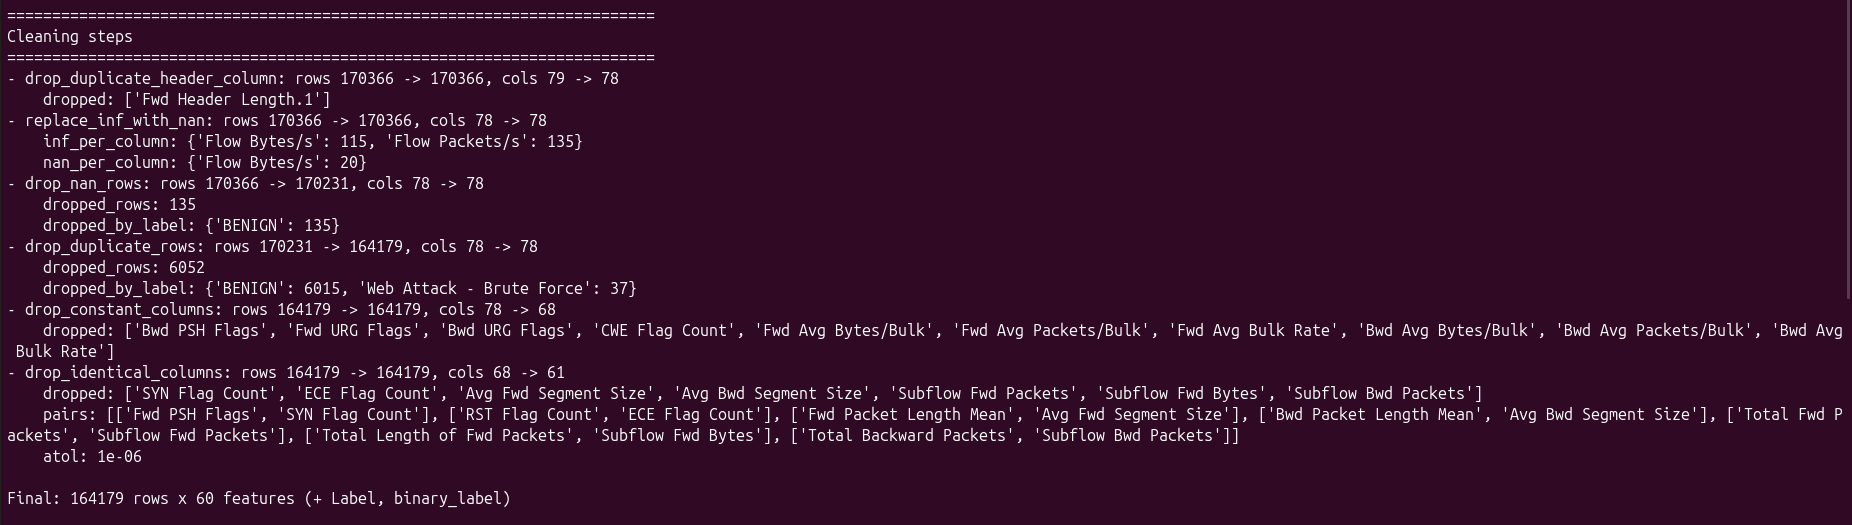
\includegraphics[width=0.8\linewidth]{SS20.png}
	\caption{Cleaning steps as logged by the pre-processing script (cf.\ Table~\ref{tab:t3cleaning}).}
	\label{fig:ss20}
\end{figure}

\begin{table}[ht]
	\centering\small
	% AUTO-GENERATED by scripts/make_report_tables.py from outputs/task3/cleaning_report.json -- do not edit
\begin{tabularx}{\linewidth}{lX}
\toprule
Kind & Columns \\
\midrule
Constant (10) & \texttt{Bwd PSH Flags}, \texttt{Fwd URG Flags}, \texttt{Bwd URG Flags}, \texttt{CWE Flag Count}, \texttt{Fwd Avg Bytes/Bulk}, \texttt{Fwd Avg Packets/Bulk}, \texttt{Fwd Avg Bulk Rate}, \texttt{Bwd Avg Bytes/Bulk}, \texttt{Bwd Avg Packets/Bulk}, \texttt{Bwd Avg Bulk Rate} \\
\midrule
Identical & \texttt{Fwd PSH Flags} $\to$ \texttt{SYN Flag Count} (dropped) \\
Identical & \texttt{RST Flag Count} $\to$ \texttt{ECE Flag Count} (dropped) \\
Identical & \texttt{Fwd Packet Length Mean} $\to$ \texttt{Avg Fwd Segment Size} (dropped) \\
Identical & \texttt{Bwd Packet Length Mean} $\to$ \texttt{Avg Bwd Segment Size} (dropped) \\
Identical & \texttt{Total Fwd Packets} $\to$ \texttt{Subflow Fwd Packets} (dropped) \\
Identical & \texttt{Total Length of Fwd Packets} $\to$ \texttt{Subflow Fwd Bytes} (dropped) \\
Identical & \texttt{Total Backward Packets} $\to$ \texttt{Subflow Bwd Packets} (dropped) \\
\bottomrule
\end{tabularx}

	\caption{Removed columns. For identical pairs, the first column is kept and the second one dropped.}
	\label{tab:t3removed}
\end{table}

After cleaning, 164,179 flows with 60 features remain, of which 2,143 (1.31\,\%) are attacks (Table~\ref{tab:t2labels}), a ratio of roughly 76 benign flows per attack. Table~\ref{tab:t3split} shows the split: the test set contains 643 attack flows, but only 6 SQL injection flows.

\begin{table}[ht]
	\centering\small
	% AUTO-GENERATED by scripts/make_report_tables.py from artifacts/clean.parquet, artifacts/split_indices.json -- do not edit
\begin{tabular}{lrr}
\toprule
Label & Train (70\,\%) & Test (30\,\%) \\
\midrule
BENIGN & 113\,425 & 48\,611 \\
Web Attack -- Brute Force & 1\,029 & 441 \\
Web Attack -- XSS & 456 & 196 \\
Web Attack -- SQL Injection & 15 & 6 \\
\midrule
\textbf{Total} & \textbf{114\,925} & \textbf{49\,254} \\
\bottomrule
\end{tabular}

	\caption{Stratified 70/30 split (\texttt{random\_state=42}).}
	\label{tab:t3split}
\end{table}

\begin{figure}[ht]
	\centering
	\begin{subfigure}[t]{0.42\linewidth}
		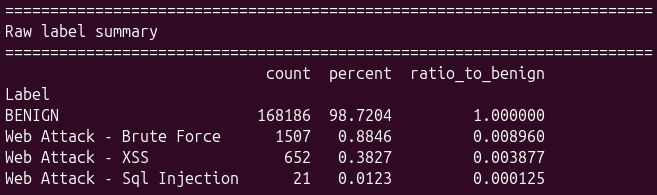
\includegraphics[width=\linewidth]{SS19.png}
		\caption{Raw labels}
	\end{subfigure}\hfill
	\begin{subfigure}[t]{0.42\linewidth}
		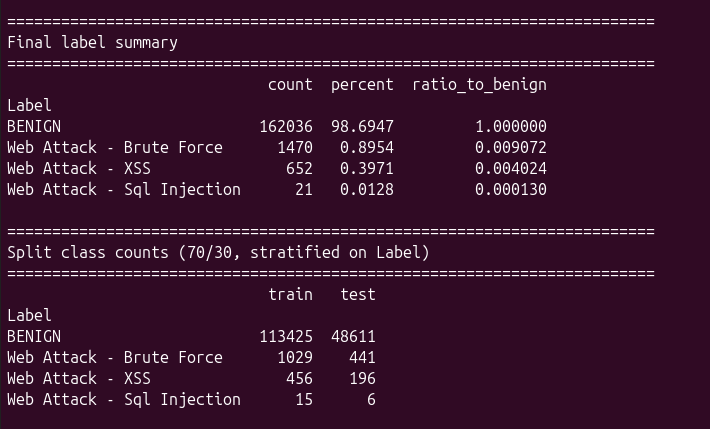
\includegraphics[width=\linewidth]{SS21.png}
		\caption{Labels after cleaning and the 70/30 split}
	\end{subfigure}
	\caption{Label analysis as printed by the pre-processing script (cf.\ Tables~\ref{tab:t2labels} and~\ref{tab:t3split}).}
	\label{fig:ss19}
\end{figure}

Table~\ref{tab:t3scaling} shows six features before and after scaling (training set). Across all 60 training columns, the scaled minimum is exactly 0 and the maximum 1 (up to floating-point rounding). The heavy-tailed durations, with maxima near the 120\,s timeout, end up with small means after scaling.

\begin{table}[ht]
	\centering\small
	% AUTO-GENERATED by scripts/make_report_tables.py from outputs/task3/describe_train_{before,after}_scaling.csv -- do not edit
\begin{tabular}{lrrrrrr}
\toprule
 & \multicolumn{3}{c}{Before scaling} & \multicolumn{3}{c}{After scaling} \\
\cmidrule(lr){2-4}\cmidrule(lr){5-7}
Feature & Min & Max & Mean & Min & Max & Mean \\
\midrule
\texttt{Init\_Win\_bytes\_backward} & $-$1 & 65\,535 & 2\,493 & 0 & 1 & 0.0381 \\
\texttt{Init\_Win\_bytes\_forward} & $-$1 & 65\,535 & 6\,354 & 0 & 1 & 0.0970 \\
\texttt{Destination Port} & 0 & 65\,529 & 8\,152 & 0 & 1 & 0.1244 \\
\texttt{Flow Duration} & $-$1 & 119\,999\,993 & 12\,876\,964 & 0 & 1 & 0.1073 \\
\texttt{Bwd IAT Total} & 0 & 120\,000\,000 & 11\,635\,099 & 0 & 1 & 0.0970 \\
\texttt{PSH Flag Count} & 0 & 1 & 0.2469 & 0 & 1 & 0.2469 \\
\bottomrule
\end{tabular}

	\caption{Six example features of the training set before and after min-max scaling.}
	\label{tab:t3scaling}
\end{table}

Table~\ref{tab:t3top20} lists the 20 selected features per target and Figure~\ref{fig:fsbin} shows the binary scores. The two lists share 18 of 20 features: only \texttt{Fwd IAT Total} and \texttt{Flow Duration} are specific to the binary target, and only \texttt{Average Packet Size} and \texttt{Bwd Packet Length Std} to the multiclass target. The scores are dominated by the top three features (above 1,600 each, against less than 250 for the rest), which is why ranks 6--20 look similar on the linear axis.

\begin{table}[ht]
	\centering\small
	% AUTO-GENERATED by scripts/make_report_tables.py from outputs/task3/feature_scores_{binary,multiclass}.csv -- do not edit
\begin{tabular}{rlrlr}
\toprule
Rank & Binary feature & $\chi^2$ & Multiclass feature & $\chi^2$ \\
\midrule
1 & \texttt{Init\_Win\_bytes\_backward} & 4525.18 & \texttt{Init\_Win\_bytes\_backward} & 4596.70 \\
2 & \texttt{PSH Flag Count} & 2928.73 & \texttt{PSH Flag Count} & 2937.06 \\
3 & \texttt{Init\_Win\_bytes\_forward} & 1616.52 & \texttt{Init\_Win\_bytes\_forward} & 1620.67 \\
4 & \texttt{ACK Flag Count} & 238.36 & \texttt{ACK Flag Count} & 246.02 \\
5 & \texttt{Destination Port} & 185.37 & \texttt{Destination Port} & 185.37 \\
6 & \texttt{Bwd IAT Total} & 100.41 & \texttt{Bwd IAT Total} & 100.44 \\
7 & \texttt{Down/Up Ratio} & 75.32 & \texttt{Down/Up Ratio} & 77.20 \\
8 & \texttt{Fwd IAT Std} & 68.76 & \texttt{Fwd IAT Std} & 70.42 \\
9 & \texttt{Fwd PSH Flags} & 68.03 & \texttt{URG Flag Count} & 69.62 \\
10 & \texttt{Bwd Packet Length Min} & 56.82 & \texttt{Fwd PSH Flags} & 68.03 \\
11 & \texttt{Idle Max} & 49.80 & \texttt{Bwd Packet Length Min} & 56.82 \\
12 & \texttt{Idle Mean} & 48.52 & \texttt{Idle Max} & 49.80 \\
13 & \texttt{Idle Min} & 46.57 & \texttt{Idle Mean} & 48.52 \\
14 & \texttt{URG Flag Count} & 44.97 & \texttt{Bwd Packet Length Std} & 47.63 \\
15 & \texttt{Packet Length Mean} & 41.21 & \texttt{Idle Min} & 46.57 \\
16 & \texttt{min\_seg\_size\_forward} & 40.12 & \texttt{Packet Length Mean} & 42.83 \\
17 & \texttt{Bwd Packet Length Mean} & 39.02 & \texttt{Bwd Packet Length Mean} & 41.50 \\
18 & \texttt{Bwd IAT Max} & 38.44 & \texttt{min\_seg\_size\_forward} & 40.12 \\
19 & \texttt{Fwd IAT Total} & 38.11 & \texttt{Average Packet Size} & 39.13 \\
20 & \texttt{Flow Duration} & 37.96 & \texttt{Bwd IAT Max} & 38.67 \\
\bottomrule
\end{tabular}

	\caption{The 20 best features by $\chi^2$ score (min-max-scaled training set), for the binary and the multiclass target.}
	\label{tab:t3top20}
\end{table}

\begin{figure}[ht]
	\centering
	\begin{subfigure}[t]{0.42\linewidth}
		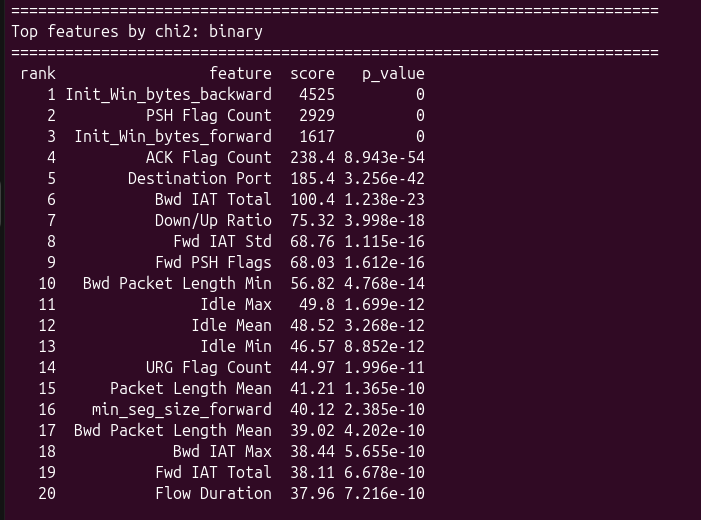
\includegraphics[width=\linewidth]{SS22.png}
		\caption{Binary target}
	\end{subfigure}\hfill
	\begin{subfigure}[t]{0.42\linewidth}
		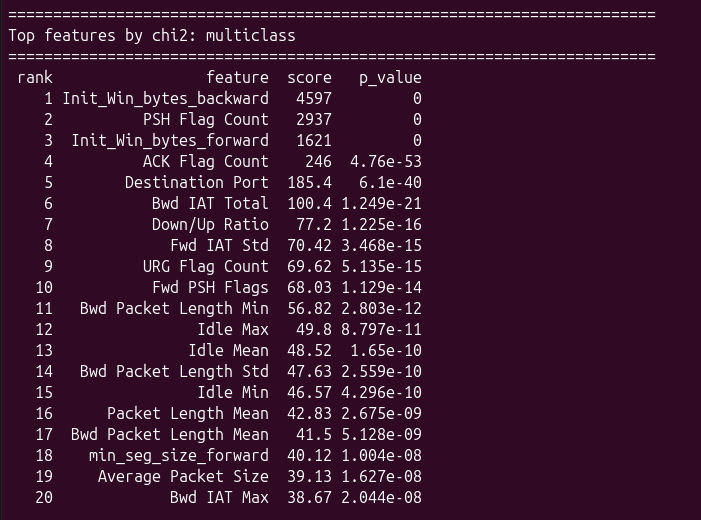
\includegraphics[width=\linewidth]{SS23.png}
		\caption{Multiclass target}
	\end{subfigure}
	\caption{The 20 best features by $\chi^2$ as printed by the pre-processing script (cf.\ Table~\ref{tab:t3top20}).}
	\label{fig:ss22}
\end{figure}

\begin{figure}[ht]
	\centering
	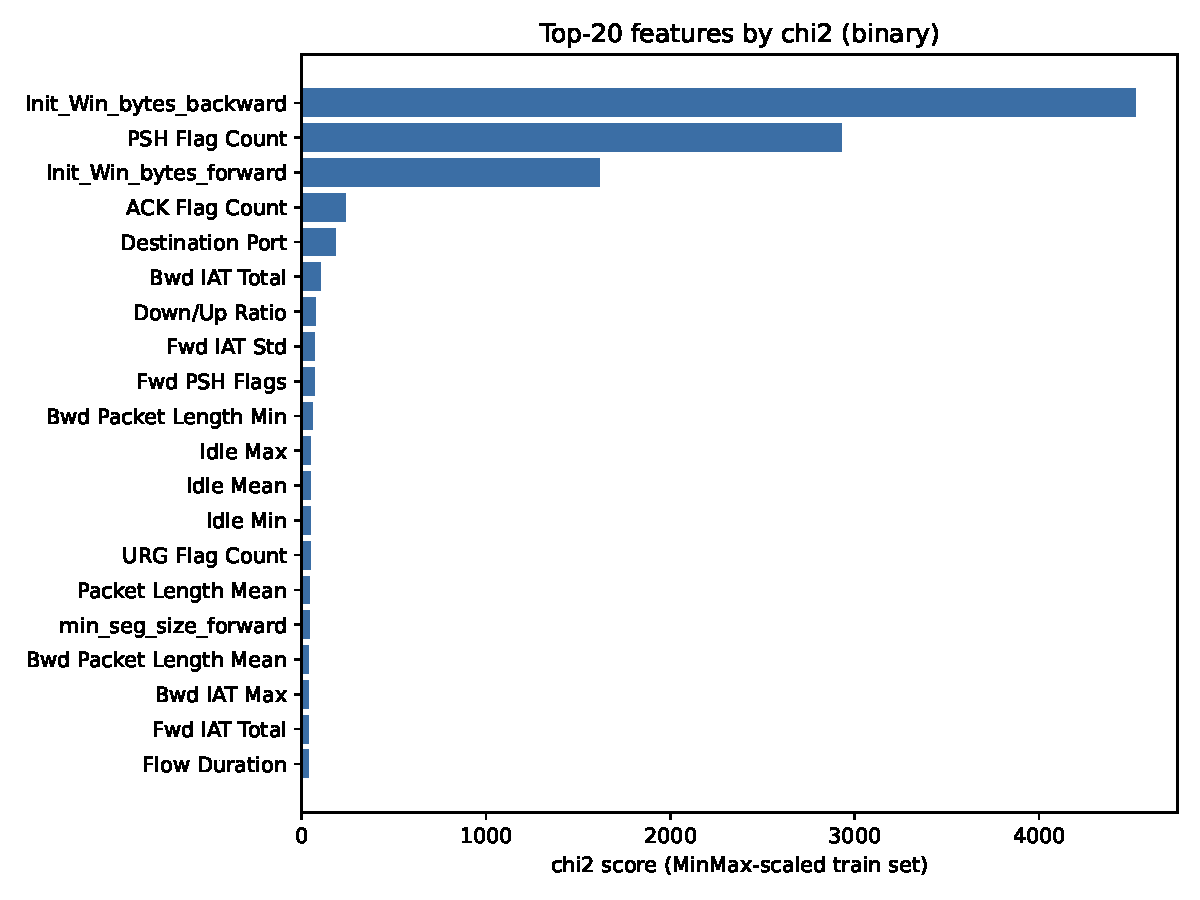
\includegraphics[width=0.75\linewidth]{feature_scores_binary.pdf}
	\caption{Top-20 flow features by $\chi^2$ score for binary classification (BENIGN vs.\ ATTACK), computed on the min-max-scaled training set.}
	\label{fig:fsbin}
\end{figure}


\section{Interpretation}\label{sec:t3-interp}

The ranking tells us what the data lets a model learn, and some of it is testbed-specific. The initial TCP window sizes (\texttt{Init\_Win\_bytes\_backward} and \texttt{\_forward}) dominate, but they depend on the operating systems and TCP stacks of the hosts in the 2017 testbed, not on the attack. \texttt{Destination Port} is a shortcut: every attack targets port 80, so a model can learn ``port 80 is suspicious'' instead of the attack behavior. The flag features (\texttt{PSH}, \texttt{ACK}, \texttt{URG}, \texttt{Fwd PSH Flags}) capture HTTP request and response patterns, and the timing features (\texttt{IAT}, \texttt{Idle}, \texttt{Flow Duration}) plausibly capture the regular pacing of the automated attacks. We expect the testbed-specific features to generalize poorly to our own traffic. The $\chi^2$ test on min-max-scaled continuous data is also only a heuristic: it treats scaled values like frequencies, and heavy-tailed features such as \texttt{Flow Bytes/s} are squeezed towards 0, which lowers their scores. The ranking therefore depends on the scaling. The multiclass ranking is given in the right half of Table~\ref{tab:t3top20}.

\FloatBarrier
